\section{Reformulations for TDA} \label{sec:tda}

In last section we have exposed the original optimal transport problem where the objetive was to measure distance between probability measures. We will now define a new Wasserstein distance, inspired in the original one, looking forward to measure the distance between persistence diagrams. In \ref{sec:wp-persistance} we make a brief introduction to Algebraic Topology and TDA concepts required to define our new Wasserstein distance. We also check that it is actually a distance between persistence diagrams. In \ref{sec:embedding} and we will conclude with the main result of this thesis: the existence of an isometric embedding from a separable metric space into the space of persistence diagrams.

\subsection{Wasserstein distance over persistence diagrams} \label{sec:wp-persistance}
We will denote the strict upper triangular region of the Euclidean plane as $ \upr := \{(x, y) \in \R^2 : x < y\} $, and the diagonal of the plane as $ \Delta := \{(x, y) \in \R^2 : x = y\}$.

\begin{definition}[Persistence diagram]
    Let $ I $ be a countable set. A {\it persistence diagram} is a function $ D: I \to \upr $.
\end{definition}

\begin{definition}[Partial matching]
    Let $ D_1: I_1 \to \upr $ and $ D_2: I_2 \to \upr $ be persistence diagrams. A {\it partial matching} between $ D_1 $ and $ D_2 $ is the triple $ (I_1', I_2', f) $ such that $ f: I_1' \to I_2' $ is a bijection with $ I_1' \subseteq I_1 $ and $ I_2' \subseteq I_2 $.
\end{definition}

Instead of probability measures, now we are actually dealing with countable sets of points in $ \R $. We will make use of the $ l^p $ norm at countable spaces to measure the distance between matched pairs and the distance between unmatched pairs and the diagonal $ \Delta $. For a more detailed explanation of Lebesgue measures check \cite{rudin}[Definition 3.7]. This norm is named after Pafnuty Chebyshev.

\begin{definition}[Chebyshev distance]
    Let $ a, b \in \R^2 $ with $a = (a_x, a_y) $ and $ b = (b_x, b_y) $. The {\it Chebyshev distance} is defined as
    $$
        d_\infty(a, b) := ||a-b||_{\infty} := \max \{|a_x - b_x|, |a_y - b_y|\}.
    $$
\end{definition}

To define our adapted Wasserstein distance we need to check how Chebyshev distance measures distances between points of $ \upr $ and $ \Delta $.

\begin{proposition} \label{prop:distance-delta}
    If $ a = (a_x, a_y) \in \upr $, then $ d_\infty(a, \Delta) = \inf_{t \in \Delta} d_\infty(a, t) = \frac{a_y - a_x}{2} $.
\end{proposition}
\begin{proof}
    The $ t $ which minimizes the distance is the midpoint of $ a_x $ and $ a_y $, that is $t = \left(\frac{a_x+a_y}{2}, \frac{a_x+a_y}{2}\right)  $. Then,
    \begin{align*}
        \left| a_x - \frac{a_x+a_y}{2} \right| = \left| \frac{a_x-a_y}{2}\right| = \left| \frac{a_y-a_x}{2}\right| = \left| a_y - \frac{a_x+a_y}{2} \right|,
    \end{align*}
    and as $ a_y > a_x $ we have
    \begin{align*}
        d_\infty(a, t) = \left|\frac{a_y - a_x}{2}\right| = \frac{a_y - a_x}{2}.
    \end{align*}
\end{proof}

We now verify that the upper triangular region of the Euclidean plane with the Chebyshev distance adapted to measure distances in $ \Delta $ is a metric space.
\begin{proposition}
    $ d_\infty $ is a distance in $ \upr $ with the diagonal $ \Delta $
\end{proposition}
\begin{proof}
    For points $ a, b \in \upr \subset \R^2 $, $ d_\infty $ is a distance as usual Lebesgue norms are well defined. See \cite{rudin}[Chapter 3]. To verify that the metric requirements are fulfilled for $ d_\infty(a, \Delta) $, it is enough to consider $ t = \frac{a_y - a_x}{2} $ as in Proposition \ref{prop:distance-delta}.
\end{proof}

\begin{definition}[$p$-cost] \label{def:pcost}
    Let $ D_1: I_1 \to \upr $ and $ D_2: I_2 \to \upr $ be persistence diagrams. Let $ (I_1', I_2', f) $ be a partial matching between them. If $ p < \infty $, the {\it $p$-cost of $ f $} is defined as
    \begin{align*}
        \costp(f) := \bigg(&\sum_{i \in I_1'} d_\infty(D_1(i), D_2(f(i)))^p \\
        &+ \sum_{i \in I_1 \setminus I_1'} d_\infty(D_1(i), \Delta)^p \\
        &+ \sum_{i \in I_2 \setminus I_2'} d_\infty(D_2(i), \Delta)^p \bigg)^{\frac{1}{p}}.
    \end{align*}
    For $ p = \infty $, the {\it $\infty$-cost of $ f $} is defined as
    \begin{align*}
        \costi(f) := \max \bigg\{&\sup_{i \in I_1'} d_\infty(D_1(i), D_2(f_i)), \\
        &\sup_{i\in I_1 \setminus I_1'} d_\infty(D_1(i), \Delta), \\
        &\sup_{i\in I_2 \setminus I_2'} d_\infty(D_2(i), \Delta)\bigg\}.
    \end{align*}
\end{definition}

\begin{definition}[p-Wasserstein distance] \label{def:Wasserstein}
    Let $ D_1, D_2 $ be persistence diagrams. Let $ 1 \leq p \leq \infty $. Define
    $$
        \twdp (D_1, D_2) = \inf \{\costp(f) : f \text{ is a partial matching between } D_1 \text{ and } D_2 \}.
    $$
    Let $ \emptyset $ denote the unique persistence diagram with empty indexing set. Let $ (\dgmp, \wdp) $ be the space of persistence diagrams $ D $ that satisfy $ \twdp(D, \emptyset) < \infty $ modulo the equivalence relation $ D_1 \sim D_2 $ if $ \twdp (D_1, D_2) = 0 $. The metric $ \wdp $ is called the {\it $p$-Wasserstein distance}.
\end{definition}

\begin{definition}[Bottleneck distance]
    In the conditions of Definition \ref{def:Wasserstein}, if $ p = \infty $, the metric $ \wdi $ is called the {\it bottleneck distance}.
\end{definition}

\begin{proposition} \label{prop-empty-mathing-distance}
    There is only one matching between $ D: I \to \upr $ and $ \emptyset $. Hence, if $ p \leq \infty $,
    $$
        \twdp(D, \emptyset) = \left(\sum_{i\in I} d_\infty(D(i), \Delta)^p\right)^{\frac{1}{p}},
    $$
    and, if $ p = \infty $,
    $$
        \twdi(D, \emptyset) = \sup_{i\in I} d_\infty(D_1(i), \Delta)
    $$
\end{proposition}
\begin{proof}
    Let $ I' \subseteq D $. If $ f $ is a partial matching between $ D $ and $ \emptyset $, means that $ f(I') = \emptyset$ is a bijection. That is only posible if $ I' = \emptyset $ too. Therefore $ I \setminus I' = I \setminus \emptyset = I $ and following Definition \ref{def:pcost} we conclude our proof.
\end{proof}

Next proposition will prove that, in indeed, the space of persistence diagrams with the $p$-Wasserstein distance $(\dgmp, \wdp)$ is a metric space. Its proof is usually omitted in literature, as it based on the simple fact that $ d_\infty $ is a distance. We will give, however, an step by step version here.

\begin{proposition}
    $\wdp$ is a distance on the space $ (\dgmp, \wdp) $.
\end{proposition}
\begin{proof}
    Let $ D_1, D_2, D_3 \in \dgmp$, with $ 1 \leq p \leq \infty $.

    First of all, $ \wdp (D_1, D_2) \geq 0 $ because $ d_\infty \geq 0 $. $ \wdp (D_1, D_2) = 0 $ if and only if $ \twdp (D_1, D_2) = 0 $. Thus, because of the equivalence relationship used to define $ \wdp $, it has to be $ D_1 \sim D_2 $.

    To check symmetry, note that every partial matching $ f $ is bijective, therefore $ f^{-1} $ is a partial matching. But, for all $ i \in I_1'$, exists $ j \in I_2' $ such that $ f(i) = j $ and
    \begin{align*}
        d_\infty (D_1(i), D_2(f(i))) = d_\infty (D_2(f(i)), D_1(i)) = d_\infty (D_2(j), D_1(f^{-1}(j))).
    \end{align*}
    Then, $ \costp(f) = \costp(f^{-1}) $ and we have
    \begin{align*}
        \wdp (D_1, D_2) &= \inf \{\costp(f) : f \text{ is a partial matching between } D_1 \text{ and } D_2 \} \\
        &= \inf \{\costp(f^{-1}) : f^{-1} \text{ is a partial matching between } D_2 \text{ and } D_1 \} \\
        &= \wdp (D_2, D_1).
    \end{align*}
    
    Finally, lets prove the triangle inequality. If $ f: I_1' \to I_2' $ is a partial matching between $ D_1 $ and $ D_2 $ and $ g: I_2' \to I_3' $ is a partial matching between $ D_2 $ and $ D_3 $, $ g \circ f: I_1' \to I_3' $ is a partial matching between $ D_1 $ and $ D_3 $ as both $ f $ and $ g $ are bijective. Computing the cost of the matchings for $ p < \infty$, we notice that
    \begin{align*}
        &\sum_{i\in I_1'} d_\infty(D_1(i), D_2(f(i))) + \sum_{i\in I_1 \setminus I_1'} d_\infty(D_1(i), \Delta) + \sum_{i\in I_2 \setminus I_2'} d_\infty(D_2(i), \Delta) \\
        + &\sum_{i\in I_2'} d_\infty(D_2(i), D_3(g(i))) + \sum_{i\in I_2 \setminus I_2'} d_\infty(D_2(i), \Delta) + \sum_{i\in I_3 \setminus I_3'} d_\infty(D_3(i), \Delta) \\
        \geq &\sum_{i\in I_1'} d_\infty(D_1(i), D_3(g \circ f(i))) + \sum_{i\in I_1 \setminus I_1'} d_\infty(D_1(i), \Delta) + \sum_{i\in I_3 \setminus I_3'} d_\infty(D_3(i), \Delta)
    \end{align*}
    as $ d_\infty(D_1(i), D_2(f(i))) + d_\infty(D_2(f(i)), D_2(g(f(i)))) \geq d_\infty(D_1(i), D_3(g \circ f(i))) $ using the triangle inequality of $ d_\infty $. Therefore, for all partial matchings $ f $ and $ g $ as described, we have $ \costp (f) + \costp (g) \geq \costp (g \circ f) $. Using the same reasoning, por $ p = \infty $ we also obtain $ \costi (f) + \costi (g) \geq \costi (g \circ f) $. Hence, we have verified that
    \begin{align*}
        \wdp(D_1, D_2) + \wdp(D_2, D_3) \geq \wdp(D_1, D_3).
    \end{align*}
\end{proof}

\begin{figure}[h] \label{fig:1}
    \centering
    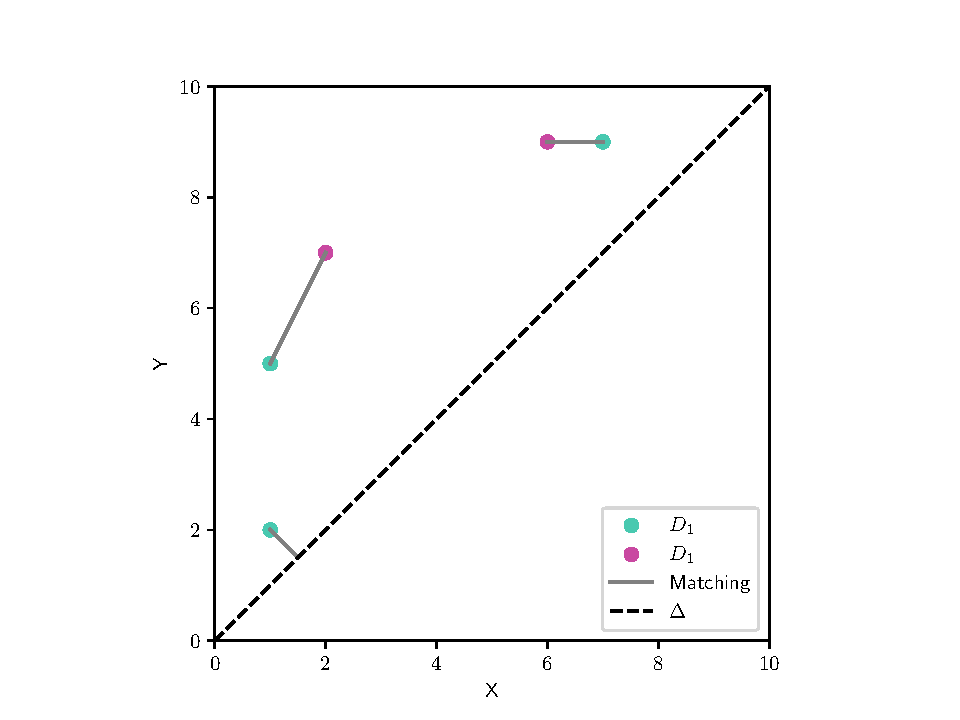
\includegraphics[width=8cm]{Figures/figure-1.pdf}
    \caption{Wasserstein distance}
\end{figure}

\subsection{Metric spaces into persistence diagrams} \label{sec:embedding}
\begin{definition}[Isometric embedding]
    Let $ (X, d_X), (Y, d_Y) $ be metric spaces. An {\it isometric embedding} $ \eta: (X, d_X) \to (Y, d_Y) $ is a mapping that satisfies
    $$
        d_X(x_1, x_2) = d_Y(\eta(x_1), \eta(x_2))
    $$
    for all $x_1, x_2 \in X$.
\end{definition}

\begin{definition}[Ball in persistence diagrams]
    Let $ 1\leq p \leq \infty $. Let $ D_0 \in \dgmp $. The {\it ball} at the space of persistence diagrams is defined as $ B_p(D_0, r) := \{D \in \dgmp : w_p(D, D_0) < r \} $.
\end{definition}

\begin{theorem}[Isometric embedding of metric spaces into persistence diagrams]
    Let $ (X, d) $ be a separable, bounded metric space. Then there exists an isometric embedding to the space of persistence diagrams $ \eta: (X, d) \to (\dgmi, \wdi)$ such that $ \eta(X) \subseteq B(\emptyset, \frac{3c}{c}) \backslash B(\emptyset, c) $.
\end{theorem}

\begin{proof}
    We will follow the procedure followed in \cite{bubenik}[Theorem 19]. As $ (X, d) $ is bounded, we can let $ c > \sup \{d(x, y): \  x, y \in X\} $. As $ (X, d) $ is separable, we can take $ \{x_k\}_{k=1}^\infty $, a countable, dense subset of $ (X, d) $. Consider
    \begin{align*}
        \eta: (X, d) &\to (\dgmi, \wdi) \\
        x &\mapsto \{(2c(k-1), 2ck + d(x, x_k))\}_{k=1}^\infty
    \end{align*}
    For any $ x \in X $ and $ k \in \N$,
    \begin{align*}
        d_\infty((2c(k-1), 2ck + d(x, x_k)), \Delta) 
        &= \frac{2ck + d(x, x_k) - 2c(k-1)}{2} \\
        &= c + \frac{d(x, x_k)}{2} \\
        &< c + \frac{c}{2} = \frac{3c}{2}.
    \end{align*}
    Because of Proposition \ref{prop-empty-mathing-distance}, for every $ x \in X $, $ \twdi(\eta(x), \emptyset) < \infty $ and $ \eta $ is well defined. Note that
    \begin{align*}
        \wdi(\eta(x), \emptyset) = \sup_{1 \leq k < \infty} d_\infty((2c(k-1), 2ck + d(x, x_k)), \Delta),
    \end{align*}
    so $ \eta(x) \in B(\emptyset, \frac{3c}{c}) \backslash B(\emptyset, c)$.

    Let $ \eta(x) $ and $ \eta(y) $ two equivalence classes of $ (\dgmi, \wdi) $. Choose the representative diagrams $D_x : \N \to \upr $ and $D_y : \N \to \upr $ and consider the partial matching $ (\N, \N, \operatorname{id}_\N) $. With it, for every $ k \in \N $, $ (2c(k-1), 2ck + d(x, x_k)) $ is matched with $ (2c(k-1), 2ck + d(y, x_k)) $. The Chebyshev distance between those points is
    \begin{align*}
        d_\infty(D_x(k), D_y(k)) 
        &= \max \big\{|2c(k-1) - 2c(k-1)|, \\
        &\quad |2ck + d(x, x_k) - b_y - (2ck + d(y, x_k))| \big\} \\
        &= \max \{0, |d(x, x_k) - d(y, x_k)|\} \\
        &= |d(x, x_k) - d(y, x_k)|.
    \end{align*}
    Hence, because of the triangle inequality, the cost of this partial matching is
    \begin{align*}
        \costi(\operatorname{id}_\N) = \sup_k |d(x, x_k - d(y, x_k)) \leq d(x, y).
    \end{align*}
    Since $ \{ x_k \}_{k=1}^\infty $ is dense, for every $ \epsilon > 0 $, there exist a $ k \in \N $ such that $ d(x, x_k) \leq \epsilon $, so
    \begin{align*}
        |d(x, x_k) - d(y, x_k)| 
        &\geq d(y, x_k) - d(x, x_k) \\
        &= d(y, x_k) + d(x, x_k) - d(x, x_k) - d(x, x_k) \\
        &\geq d(x, y) - 2d(x, x_k) \\
        &> d(x, y) - 2\epsilon.
    \end{align*}
    Therefore, $ \sup_k |d(x, x_k - d(y, x_k)) \geq d(x, y) $ and
    \begin{align*}
        \costi(\operatorname{id}_\N) = \sup_k |d(x, x_k - d(y, x_k)) = d(x, y).
    \end{align*}
    Suppose $ I, J \subseteq \N $ and $ (I, J, f) $ is a different partial matching between $ D_x $ and $ D_y $. Then there exist a $ k \in \N $ such that either $ k \notin I $ or $ k \in I $ and $ f(k) = k \neq k $. If $ k \notin I $, then
    \begin{align*}
        \costi(f) \geq d_\infty((2c(k-1), 2ck + d(x, x_k)), \Delta) \geq c.
    \end{align*}
    If $ k \in I$ and $ f(k) = k \neq k $, then
    \begin{align*}
        \costi(f) \geq || (2c(k-1), 2ck + d(x, x_k)) - (2c(k'-1), 2ck' + d(x, x_{k'}))||_\infty \geq 2 \epsilon.
    \end{align*}
    Hence, $ \costi(f) \geq c > d(x, y)$ and $d(x,y) = \wdi(\eta(x), \eta(y)) $, proving that $ \eta $ is an isometric embedding of a metric space into the space of persistence diagrams.
\end{proof}

\begin{figure}[h] \label{fig:2}
    \centering
    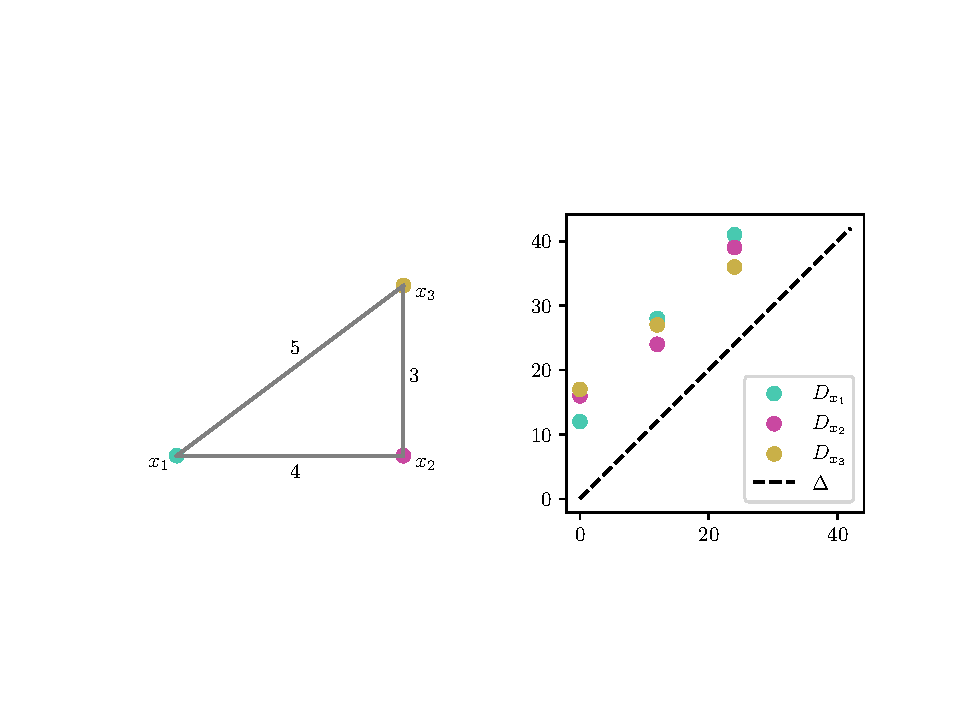
\includegraphics[width=8cm]{Figures/figure-2.pdf}
    \caption{Isometric embeeding}
\end{figure}